\chapter{Représentation des cartes de Kohonen}
\graphicspath{{03-Representation/}}

\minitoc
\section{Représentation et explicabilité des cartes de Kohonen}

Les algorithmes d'apprentissage sont généralement composés de structures complexes. Leur règles d'évolution et leur structures sont certes connues et conçues par leur développeur, mais leur état au cours de l'apprentissage dépend de tellement de paramètres que le concepteur ne peut plus prévoir son état - c'est bien la le rôle d'un algorithme. Cet état doit alors être étudié et observé au même titre qu'un processus observé dans la nature. La représentation d'un algorithme d'apprentissage est ainsi un défi posé depuis quelques années. 

Lorsqu'on s'intéresse à des algorithmes supervisés, dans lesquels l'évolution dépend d'une fonction de coût et d'un objectifs, des métriques assez évidentes existent, en s'intéressant à l'erreur de prédiction. Mais même en situation supervisée, le problème est largement ouvert quand il s'agit de comprendre les mécanismes d'apprentissage à l'oeuvre dans la structure. Cette question de représentation est notamment soulevée dans l'étude de l'explicabilité de l'intelligence artificielle. Quand on s'intéresse aux algorithmes non-supervisés, la question de représentation de l'algorithme devient centrale: \emph{Que cherche-t-on à représenter et comment déterminer si on en a extrait une bonne représentation ?}

En particulier, les  "Est ce que les prototypes ont extrait une information pertinente des données" n'a en fait que des réponses partielles dans la littérature. Il s'agit d'abord de déterminer ce qu'on cherche à apprendre dans un cas spécifique. Nous nous poserons ainsi cette question pour l'architecture CxSOM. 
%
%Dans un cas plus général de cartes auto-organisatrices, telles que celles agissant dans CxSOM, l'apprentissage repose sur des calculs d'activités et un processus de relaxation. Ces activités n'ont pas forcément un pendant graphique. De ce fait, leur représentation graphique mérite une analyse plus approfondie que dans le cas de cartes classiques. 



\subsection{Représentation classique des cartes de Kohonen}

Les cartes de Kohonen sont un algorithme d'apprentissage certes non-supervisé, mais sont particulièrement associées à une facilité de représentation et de visualisation. En effet, leur nombre réduit de prototypes et leur aspect topologique permet d'en tracer une représentation visuelle interprétable.
La manière la plus utilisée de représenter une carte de Kohonen est de tracer les poids de ses prototypes, disposés dans le graphe qu'est la carte. En fonction des dimensions des entrées, cette représentation prennent plusieurs formes. Deux exemples courants de représentation sont les suivants: 
\begin{itemize}
\item Le graphe qu'est la carte de Kohonen est représenté dans l'espace de ses positions (la grille d'indices $(i,j)$, ou une ligne indexée par $i$. Sur chaque noeud est tracé le poids correspondant. C'est le cas sur l'exemple de gauche en figure~\ref{fig:representation} dans lequel les poids des prototypes, qui sont des imagettes, sont affichés en chaque point de la grille. Si la dimension d'un poids est trop grande pour être représentée graphiquement, il est également courant de labeliser chaque prototype et d'afficher ces labels sur les noeuds de la carte, en tant que représentation.
\item Lorsque les données traitées sont des points deux ou trois dimensions, les poids des prototypes peuvent être directement tracés dans l'espace $R^2$ ou $R^3$. Ces poids sont alors reliés en fonction des positions des noeuds dans la carte, montrant ainsi la déformation de la carte dans l'espace d'entrée, c'est le cas sur l'exemple de droite en figure~\ref{fig:representation}.
\end{itemize}

\begin{figure}
\begin{minipage}{0.5\textwidth}
\centering
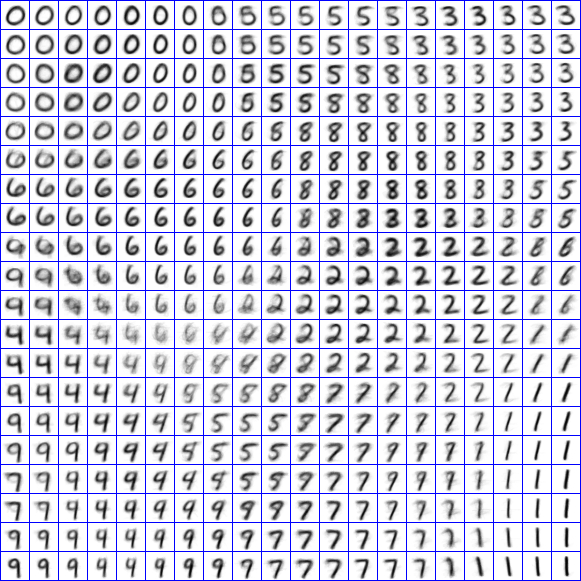
\includegraphics[width=0.5\textwidth]{digits.jpg}
\end{minipage}
\begin{minipage}{0.5\textwidth}
\centering
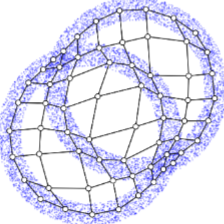
\includegraphics[width=0.5\textwidth]{points.png}
\end{minipage}
\label{fig:representation}
\caption{Représentations possible des poids d'une carte de Kohonen classiques, dans le cas d'entrées sous forme d'imagettes ou de points en deux dimensions.}
\end{figure}

On parle cependant ici d'interprétation visuelle humaine. Pour l'oeil humain, cette facilité d'interprétation est limitée à un domaine d'utilisation : celui dans lequel les éléments qui nous intéressent sont les distances euclidiennes entre les données, ou plus généralement dans lequel la distance considérée pour la mise a jour des cartes possède un aspect graphique facilement interprétable. Essayez par exemple de vous représenter des distances dans un espace non-euclidien, comme en figure~\ref{fig:non_eucl}. Savoir quels points sont les plus proches nécessite alors un effort mental important et non une seule intuition; finalement la façon la plus simple de le savoir est de faire le calcul. 
La représentation d'une carte cherche à répondre à la question: "est-ce que la carte est bien dépliée sur toutes les données ? Est-ce qu'un prototype représente correctement une donnée ?". Y répondre en visualisant ses prototypes revient au processus intellectuel suivant: l'observateur imagine une donnée, par exemple une imagette d'un chiffre à main levée, et reproduit le processus de sélection du BMU qui a eu lieu lors de l'apprentissage de la carte pour trouver le poids qui lui correspond le mieux. Via ce processus mental, on est capable d'évaluer si une carte est dépliée sur les données. 
Imaginons à présent que les distances considérées entre les éléments d'une carte ne soient plus euclidiennes: cette évaluation du dépliement de la carte repose maintenant sur soit une capacité d'abstraction phénoménale de l'observateur, soit des calculs de distances entre les points. La représentation de la carte doit ainsi être ajustée en fonction du processus d'organisation.

Finalement, pour représenter un algorithme d'apprentissage non-supervisé et en particulier une carte de Kohonen, on doit d'abord bien poser ce qu'on cherche à évaluer; ensuite, cette représentation doit être adaptée aux règles de calcul de l'algorithme, ici de l'espace de la carte. 

\begin{figure}
\begin{minipage}{0.5\textwidth}
\centering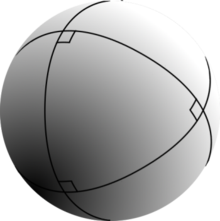
\includegraphics[width=0.5\textwidth]{sphere.png}
\end{minipage}
\begin{minipage}{0.5\textwidth}
\centering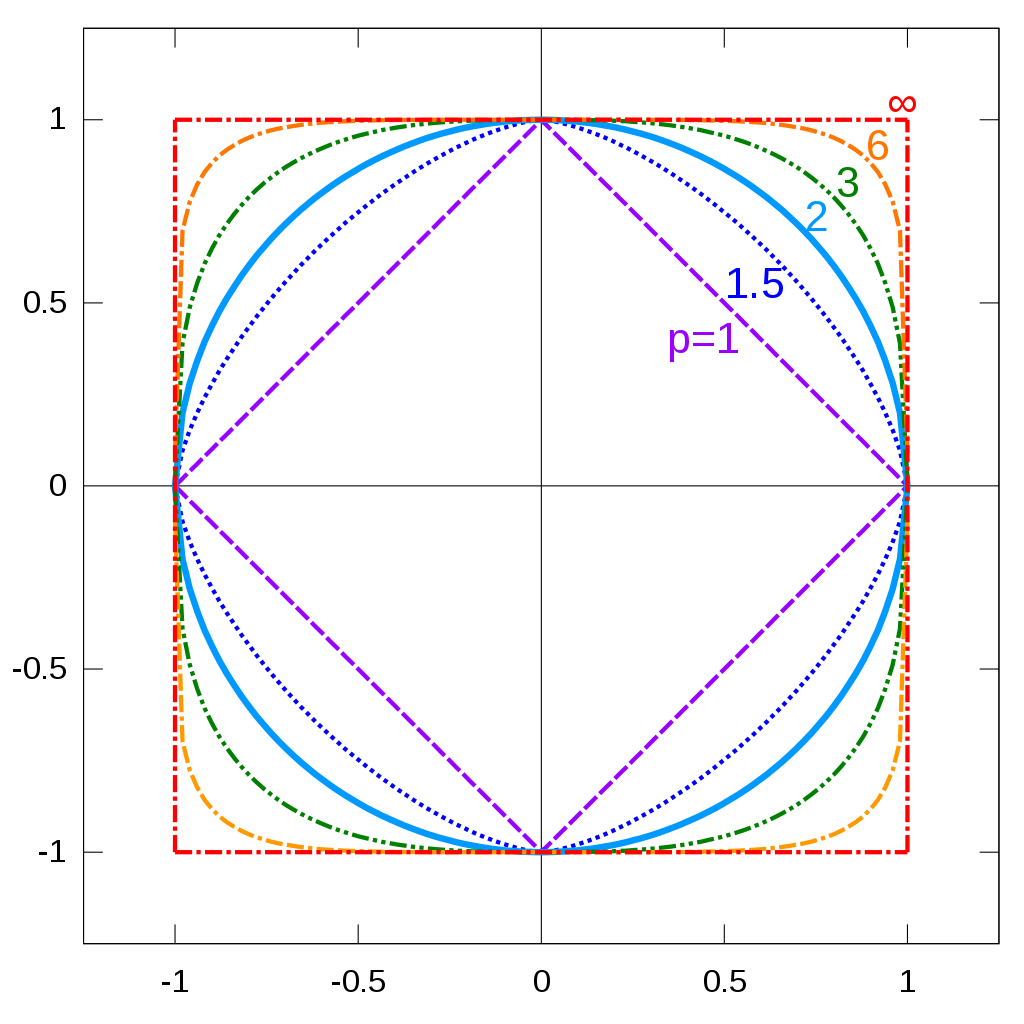
\includegraphics[width=0.7\textwidth]{norm.png}
\end{minipage}
\label{fig:non_eucl}
\caption{Appréhender les distances et les formes en géometrie sphérique n'est pas intuitif pour l'oeil humain. Le triangle de la figure à gauche possède trois angles droits. La figure de droite présente les cercles unités en deux dimensions par rapport à plusieurs normes.}
\end{figure}




\subsection{Que cherche t-on à représenter dans CxSOM ?}

Pour pouvoir étudier le comportement d'une architecture de cartes, il nous faut donc répondre à ces deux questions de représentation. 

La représentation des prototypes dans chaque carte n'est plus un bonne représentation de l'architecture.
En effet, le choix du BMU se fait suivant plusieurs activités, et plus encore, suivant un processus de relaxation. Il est bien entendu possible de tracer les poids d'une carte après apprentissage, comme représenté en figure~\ref{fig:weights}. Cependant, le processus intellectuel menant à la représentation mentale d'une carte, en regardant les poids, n'est plus possible. En imaginant une donnée, on ne pourra pas trouver le BMU selectionné. La simulation du processus d'activité et relaxation est nécessaire pour la représentation compréhensible par l'humain d'une carte au sein de CxSOM. Par ailleurs, chaque unité d'une carte a plusieurs poids. Il est donc compliqué de comprendre directement le rôle de ces poids en regardant leur valeur.
\begin{figure}
\centering
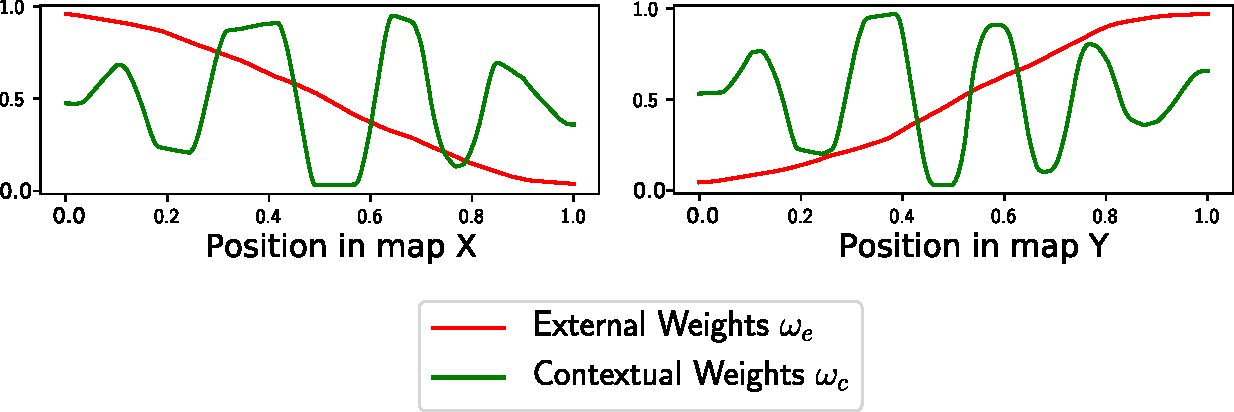
\includegraphics[width=0.7\textwidth]{weights_2.pdf}
\label{fig:weights}
\caption{Représentation des valeurs des poids d'une carte au sein de CxSOM. La seule représentation de ces poids ne suffit pas à savoir comment la carte se comporte. }
\end{figure}
De plus, la représentation visuelle des cartes d'une architecture est limitée par la dimension des entrées et la dimension des cartes. Ici s'ajoute à la dimension des entrées la dimension d'une carte et le nombre de carte. Il sera difficile de représenter graphiquement des architectures de plus de trois cartes, et encore plus lorsque les entrées sont en grande dimension. Cette difficulté de représentation soulève la nécessité de définir des valeurs indicatrices du fonctionnement de la carte, calculables en grande dimension.

Mais, qu'est ce qu'une carte \emph{qui fonctionne ?}. L'intéret de CxSOM réside dans la communication entre cartes. Représenter les cartes une à une laisse donc de coté leur connexion. Il est donc nécessaire de trouver un moyen de représenter l'architecture comme un tout.

Ce chapitre questionne donc la façon de représenter une carte de Kohonen, et plus particulièrement la façon de représenter une carte au sein d'une architecture. Nous présenterons donc en premier lieu un formalisme pour la carte et les entrées multimodales associées, et à partir de ce formalisme nous proposerons plusieurs représentations et indicateurs cherchant à comprendre ce que l'architecture apprend sur les données d'entrée, et de quelle façon. 

\section{Formalisme: variables aléatoires}

Nous introduisons dans cette section un formalisme traitant les éléments des cartes et les entrées en tant que variables aléatoires. Ce formalisme a l'avantage de à la fois clarifier les représentations, et de permettre le développement d'indicateurs statistiques sur les cartes.

\subsection{Représentation des entrées}

Les observations multimodales que l'on cherchera à apprendre par l'architecture de cartes sont notées ${X^i, i = 0 \cdots N}$ où $N$ est le nombre de modalités considérées. Lors de l'apprentissage et du test, elles sont échantillonnées; ainsi, à chaque pas de temps, l'architecture se voit présentée un vecteur $(X^0_t, \cdots, X^N_t)$.
Lorsqu'elles sont considérées en tant que \emph{entrée externe} d'une carte, on les notera plutôt ${\inpx^i, i=0 \cdots N} $, avec $i$ l'indice de la carte dont $\inpx^i$ est l'entrée.
Pour tout $i$, $X^i$ et $\inpx^i$ sont des variables aléatoires, et $\mathbf{X} = (X^0, \cdots, X^N)$ et $\mathbf{\inpx} = (\inpx^0, \cdots , \inpx^N)$ sont les vecteurs aléatoires correspondants.

Pour les entrées CxSOM, on s'intéresse à l'apprentissage de relations entre entrées. Les variables $X^i$ ne sont a priori donc pas des variables indépendantes. Afin de mieux comprendre comment les cartes apprennent des relations entre les entrées, on introduit une autre variable aléatoire $U$. Cette variable est multidimensionnelle et est choisie de façon à ce que chaque variable $X^i$ soit une fonction quelconque de la variable aléatoire $U$, et uniquement de cette variable. Il s'agit en fait d'une réduction de dimension:

\begin{equation}
\forall t, \forall i, X^i_t = f^i_t(U_t)
\label{eq:U}
\end{equation}

Cette variable traduit l'existence d'un modèle reliant les observations.
Prenons un exemple géométrique; considérons des points tirés sur un cercle quelconque dans l'espace en deux dimensions. $\mathbf{X} = (X^0,X^1)$, les coordonnées cartésiennes des points du cercle, est alors une vecteur aléatoire, dont les composantes sont les variables aléatoires $X^0,X^1$. En définissant une variable $U$ à valeurs réelles, chaque point du du cercle peut maintenant s'écrire, selon l'équation paramétrique du cercle: 
$$
 \begin{cases}
     X^0_t = r  \cos(U_t)\\
     X^1_t = r \sin(U_t)
    \end{cases}\,.
$$
$U$ représenterait ici l'angle du point sur le cercle. $U$ est une variable cachée qui \emph{réduit la dimension} du modèle. ELle contient toute l'information sur l'échantillon. 

$U$ et ${f^i}$ ne sont pas uniques. Elle sont choisies en fonction de ce qu'on cherche à traduire dans le modèle. Ainsi, pour le même ensemble de points sous forme de cercle, on peut aussi définir une variable $U$ en deux dimensions, une dimension à valeur réelles paramétrisant un demi cercle, l'autre à valeurs dans ${0,1}$ indiquant de quel coté de l'axe des abscisses on se situe.

Notons par contre que la plus petite dimension possible de $U$ dépend du degré de liberté du modèle. Si toutes les observations se situent sur une courbe de dimension 1, alors il existe une variable $U$ en une dimension satisfaisant l'équation~\ref{eq:U}. Si les observations se situent sur une surface de dimension 2, alors, $U$ sera en deux dimensions, et ainsi de suite.

\begin{figure}
\begin{minipage}{0.5\textwidth}
\centering
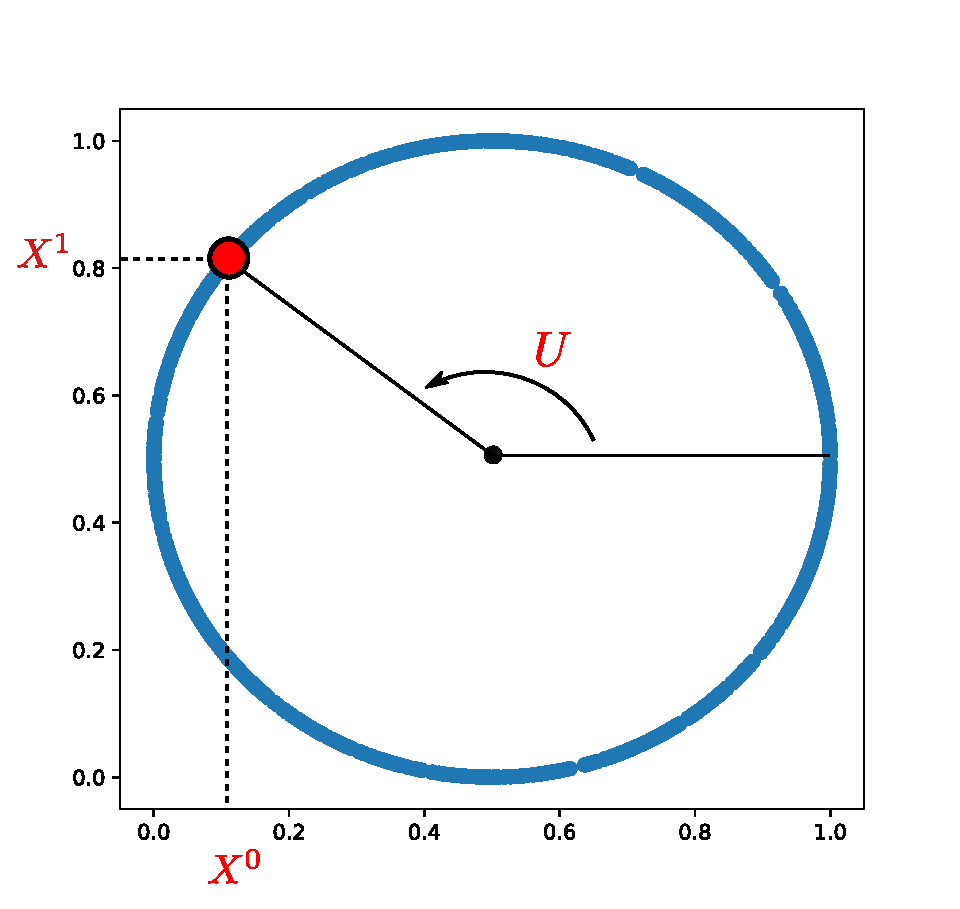
\includegraphics[width=0.6\textwidth]{cercle.pdf}
\end{minipage}
\begin{minipage}{0.5\textwidth}
\centering
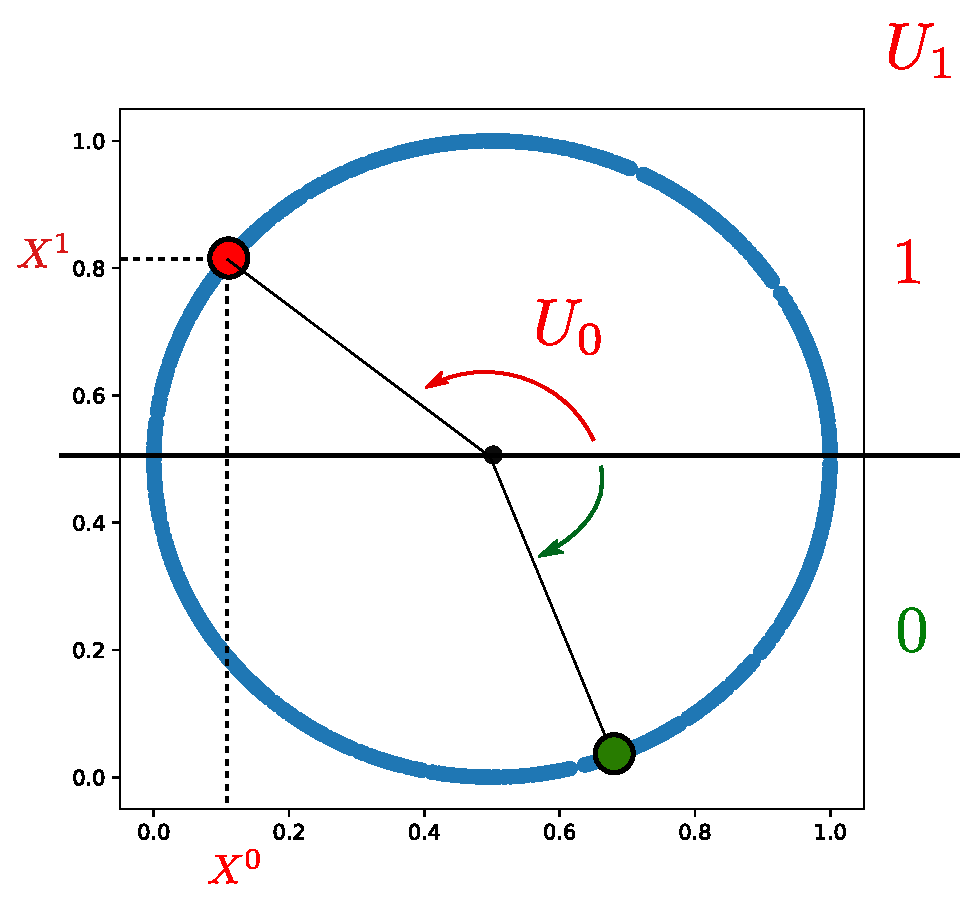
\includegraphics[width=0.6\textwidth]{cercle_2.pdf}
\end{minipage}
\caption{Exemples de paramétrisations du cercle. La paramétrisation qui traduit le plus facilement le modèle est naturellement celle dans laquelle $U$ est à valeurs réelles. Le modèle auxquelles appartiennent les modalités $X^0$ et $X^1$ est donc représenté par la variable cachée $U$.}
\end{figure}

Cette façon de représenter les entrées est-elle générale ? 


\subsection{Représentation des éléments des cartes}

Comme dans de nombreux algorithmes d'apprentissages, on peut décomposer le jeu de données d'entrée en jeu d'apprentissage et jeu de tests. Lors de la phase de test, seul le processus de recherche de la best matching unit est réalisé et la partie mise à jour des cartes de Kohonen n'est plus opérée. Dans le cadre des variables aléatoires, chaque itération est alors un tirage indépendant. Les éléments des cartes peuvent donc être considérés comme des variables aléatoire et une itération de test comme la réalisation de celles-ci. La phase de test peut être réalisée après n'importe quelle itération de l'algorithme d'apprentissage. Le processus d'apprentissage et de tests est décrit en figure~\ref{fig:flowchart}.

Nous considérerons alors plusieurs éléments des cartes en tant que variables aléatoires, notamment :  
\begin{itemize}
\item Les positions des BMUs $\bmu^0, \cdots, \bmu^N$ dans chaque carte
\item Les poids externes des BMUs $\w_e^0(\bmu^0), \cdots, \w_e^N(\bmu^N)$
\end{itemize}
Notons que tout élément d'une carte pourrait être vu de cette manière. 
Une phase de test est donc un grand nombre de réalisations d'une variable aléatoire jointe : 
$$(\inpx^0, \cdots, \inpx^N, \bmu^0, \cdots, \bmu^N, \w_e^0(\bmu^0), \cdots, \w_e^N(\bmu^N))$$
Les composantes de cette variable jointe ne sont pas indépendantes. Les représentations et indicateurs présentés ensuite chercheront à détecter et comprendre au mieux ces dépendances statistiques.

Ainsi, dans ce formalisme par variable aléatoires, à chaque pas d'apprentissage peut-être associé un ensemble de réalisations de variables aléatoires. Ceci permet alors d'utiliser des outils et métriques issus de la théorie de l'information pour qualifier l'organisation des cartes au sein de l'architecture. Cette approche ne se limite pas à l'architecture CxSOM : 
%la théorie de l'information semble être un élément intéressant à explorer pour comprendre le fonctionnement d'algorithmes non-supervisés. -> La théorie de l'information est utilisée pour comprendre des architectures informatiques, biologiques, en neuroscience .... Exemples cités dans le papier Timme2013

\begin{figure}
\centering
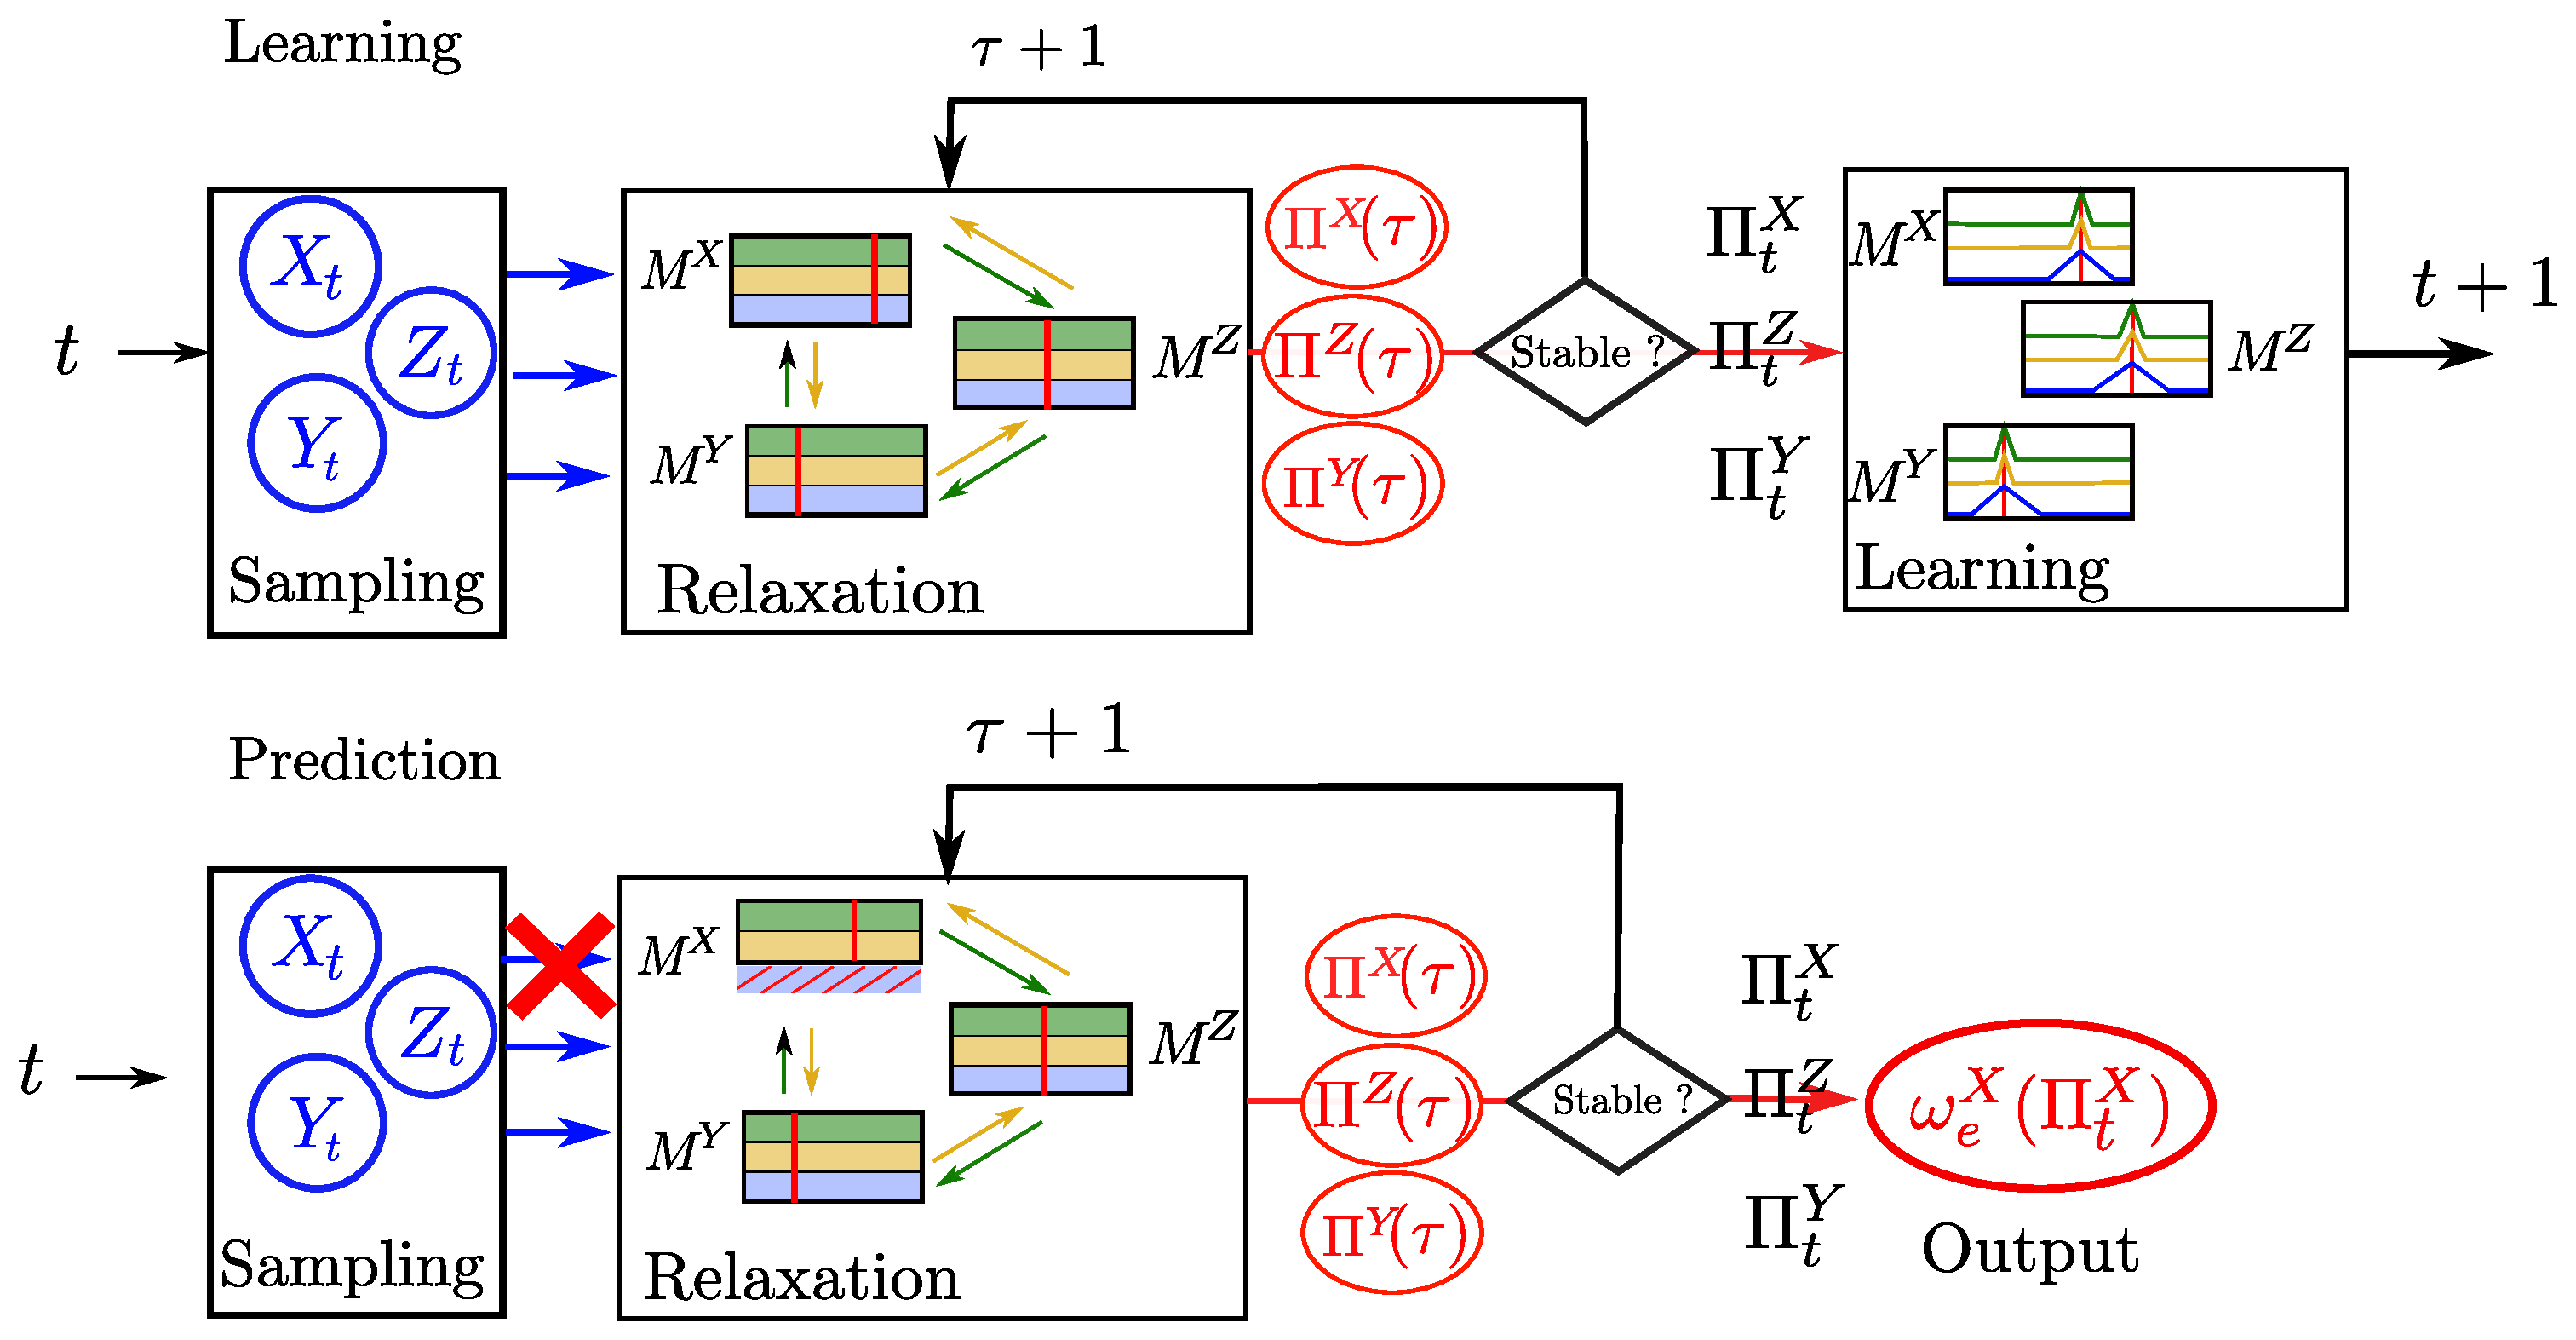
\includegraphics[width=0.7\textwidth]{learning_tests.pdf}
\caption{Schéma descriptif de l'apprentissage et des tests.}
\label{fig:flowchart}
\end{figure}


\section{Représentations graphiques}

\emph{Qu'est ce qu'une carte a appris des données ?}

Que cherche t-on à représenter dans les représentations classiques des poids des cartes de Kohonen, que ce soit sous la forme d'un tableau de prototypes ou d'une projection dans l'espace d'entrée ? On cherche en fait à visualiser comment les poids sont répartis en fonction de leur \emph{position} dans la carte. En d'autres termes, on cherche à comprendre si les positions de la carte correspondent à tous les éléments de l'espace d'entrée, si une continuité est réalisée. 
D'une façon similaire, on peut faire le choix de représenter le poids de la best matching unit par rapport à sa position. Cela donne la même représentation que le fait de tracer le poids de chaque prototype par rapport à sa position dans la carte; à la seule différence qu'elle fera la distinction entre les \emph{unités mortes de la cartes}, c'est à dire les unités qui ne sont jamais best matching unit et qui ne seront donc pas affichée dans la représentation des tests, et les autres.
Cette représentation prend en compte la façon de calculer le BMU, donc le coeur de l'algorithme.

La question de la répartition des valeurs d'une carte par rapport à la position de leur BMU va plus loin que les poids : il est intéressant d'étudier la répartition de n'importe quel élément d'une carte de cette façon, afin de comprendre 
De façon plus générale, on peut représenter, à partir d'un échantillon test, la dépendance de n'importe quelle variable par rapport à la position de la best matching unit correspondante. Nous détaillerons dans cette partie quelques représentations qui paraissent pertinentes.


\subsection{Représenter les entrées par rapport à une carte}

Représentation des entrées de test sur les poids de la carte

\subsection{Représentation de U par rapport au BMU}
\emph{Chercher à apprendre des relations entre les données}

Un des objectifs principaux de l'architecture CxSOM est d'encoder les relatations entre les données d'entrée. Il nous faut donc tracer des valeurs qui expriment cette relation. 
Expliquer mieux comment $U$ est choisi : il s'agit d'une transformation non linéaire des données sur un autre espace, dans lequel $U$.

TODO : cas des cartes 2D, cas des entrées 


\subsection{Représentation des cartes sous forme de "distortion" (trouver un mot)}



\section{Information mutuelle comme indicateur statistique}

De nombreuses valeurs ont été développées en théorie de l'information, depuis Shannon en 1948 (citer), pour mesurer des dépendances entre variables.
Lister les spécificités des mesures et dans quel cas on peut les utiliser: 
Mesure proba / estimation ( estimation en grande dimensions, etc)
Est ce que les distributions doivent etre connues ...

Exemple de domaines d'application de ces mesures

Ces mesures s'appuient sur des variables : elles ne dépendent pas du modèle. 

\subsection{Information mutuelle et entropie}

Les notions d'\emph{entropie} et les valeurs qui en sont dérivées, telle que l'\emph{information mutuelle} entre des distributions, sont des notions fondamentales de la théorie de l'information de Shannon. Ces quantités donnent des informations concernant la distribution d'une variable aléatoire.
Les formules indiquées dans ce paragraphe concernent des variables aléatoire discrètes. 
L'entropie de Shannon d'une variable aléatoire $X$, de distribution $p(X)$, est notée $H(X)$ et définie par la formule : 
$$ H(X) = - \sum_{x \in X}{p(x)\textrm{log}(p(x))}$$
Elle se mesure en $bit/symbole$ lorsque le le logarithme est en base 2, ce qui est généralement utilisé. 
L'entropie est une mesure de la quantité d'incertitude, ou de surprise, sur la valeur de la variable aléatoire $X$. Si la la distribution de probabilité de $X$ est concentrée autour d'un point, l'entropie est faible : lors d'une réalisation de $X$, l'observateur est \emph{plutôt certain} du résultat. En revanche, l'entropie est maximale lorsque lorsque $X$ suit une distribution de probabilité uniforme.
L'entropie s'interpète également comme la quantité moyenne d'information à fournir, en bits, pour coder la valeur que prend la variable $X$.
De la même manière, on peut définir l'entropie conjointe de deux variables, qui est l'entropie de leur distribution jointe, et l'entropie conditionnelle, qui est l'entropie de leurs distributions conditionnelles.

Outre les entropies jointes et conditionnelles, les relations statistques entre deux variables aléatoires peuvent être mesurées par \emph{l'information mutuelle}. Elle se définit formellement par : 
$$ I(X,Y) = \sum_{x,y \in X,Y}{p(x,y)\textrm{log}(\frac{p(x,y)}{p(x)p(y)})}$$
Cette valeur mesure la quantité d'information moyenne apportée par une réalisation de $X$ sur la réalisation de $Y$. L'information mutuelle possède notamment les propriété suivantes: 
$$I(X,Y) = 0 \Leftrightarrow \textrm{X et Y sont indépendantes}$$
Cette propriété se comprend dans la définition de $I$: si $X$ et $Y$ sont indépendantes, $p(x,y)=p(x)p(y)$ et terme $\textrm{log}(\frac{p(x,y)}{p(x)p(y)}$ est nul pour toute les valeurs de $x$ et $y$. Inversement, $I(X,Y) =0$ ssi tous les termes (positifs) de la somme sont nuls, donc si $(p(x,y)=p(x)p(y)$ pour toutes les valeurs de $X$ et $Y$. L'information mutuelle est donc aussi une mesure de la distance entre la distribution jointe de $(X,Y)$ et leur indépendance.


Elle s'exprime à partir de l'entropie : $$I(X,Y) = H(X) + H(Y) - H(X,Y) = H(X) - H(X|Y) = H(Y) - H(Y|X)$$

Elle est symétrique : $$I(X,Y) = I(Y,X)$$

Pour toute fonction $f$, $I(X,Y) \geq I(X,f(Y)$. L'égalité est atteinte ssi $f$ est \emph{bijective}. (proof?)

\subsection{Indicateur: coefficient d'incertitude.}

Lors de l'analyse de CxSOM, on souhaite comprendre l'information que portent les positions des BMUs d'une carte sur le modèle d'entrées. Nous avons défini les éléments de la carte en terme de variables aléatoire; l'information mutuelle peut alors être une représentation pertinente de l'information portée par le BMU d'une carte sur le modèle. Le modèle est représenté par la variable $(X,Y,Z)$, mais aussi par $U$. Dans ce sens, $I(\bmu, U)$ est l'information que porte le BMU d'une carte sur $U$, donc sur le modèle. 

On souhaite cependant avoir un indicateur absolu, qui permettrait, sur une échelle de 0 à 1, de quantifier à quel point un BMU porte de l'information sur $U$. On va donc normaliser l'information mutuelle $I(\bmu,U)$ par la valeur maximale qu'elle peut prendre dans notre carte.
\begin{propriete}
La valeur maximale atteinte par $I(\bmu,U)$ est $H(U)$, atteinte lorsque $U$ est fonction de $\bmu$.
\end{propriete}

\begin{proof}
Par construction, $\Pi$ est une fonction de $U$ dans une carte de Kohonen. En effet, notre algorithme est déterministe et une sortie est définie pour toute valeur de U. 
Par propriété de l'information mutuelle, pour toute fonction $f$ et variable $X,Y$, $I(X,f(Y)) \leq I(X,Y) $.
Donc, $I(U,\bmu) \leq I(U,U) = H(U)$
Cette valeur est atteinte si et seulement si $U$ et $\bmu$ sont en bijection, autrement dit, ssi $U$ est aussi une fonction de $\bmu$.
\end{proof}

Nous définissons donc un indicateur de la relation entre $U$ et un BMU comme:
\begin{equation}
UC(\bmu;U) = \frac{I(\bmu,U)}{H(U)}
\end{equation}
Ce coefficient n'est pas symétrique, et mesure donc l'information portée par le premier terme sur le second, relativement à la valeur maximale qu'elle peut prendre. Dans le cas des cartes CxSOM, $UC \in [0,1]$. 

Ce coefficient peut être élargi à plus de variables. On peut ainsi calculer UC(($\bmu^1,\bmu^2,\bmu^3),U)$ pour 3 cartes, en considérant la variable jointe $(\bmu^1,\bmu^2,\bmu^3)$.

\subsection{Estimation}

L'information mutuelle et l'entropie sont des grandeurs probabilistes. Elles sont définies à partir de la distribution des variables aléatoire. Lorsque qu'on ne connait pas les distributions, il est nécessaire d'estimer ces valeurs autrement. 
Dans le cas d'étude, les variables considérées sont 1D, et le nombre d'échantillon disponible est grand. On estime donc la distribution des variables en réalisant du \emph{binning}, et les indicateurs sont calculés à partir de cette estimation.

Limitations de cette estimation:
\begin{itemize}
\item La taille des boites doit être sélectionnée manuellement pour le moment, donc dans le cas ou on veut utiliser cet indicateur, a savoir avec $U$, $\bmu$ de plus grande dimension ou des cartes 2D, il faut un processus qui permet de choisir une bonne taille de boites.
\item En parlant plus grande dimension, on est limité dans le binning par les boites vides: la taille de l'échantillon devrait augmenter exponentiellement en fonction de la dimension pour que l'approximation d'une densité soit toujours valide. Sinon, on a trop de boites vides qui ne le snot que parce que les données sont trop éparses. Donc il faut penser à d'autres méthodes d'estimations, telles que Kraskov. Cette estimation est un problème difficile a résoudre ...
\end{itemize}

Limitation de l'estimateur : en transformant la densité continue en discrète, on perd la notion de proximité entre les valeurs de $U$ et entre les positions. Ainsi, des données dispersées autour d'un point à la position $p$ seront considérées de la même façon que si elles sont dispersée autour de deux points séparés. On a donc intérêt à trouver un indicateur qui prend en compte la proximité ...

\begin{figure}
\centering
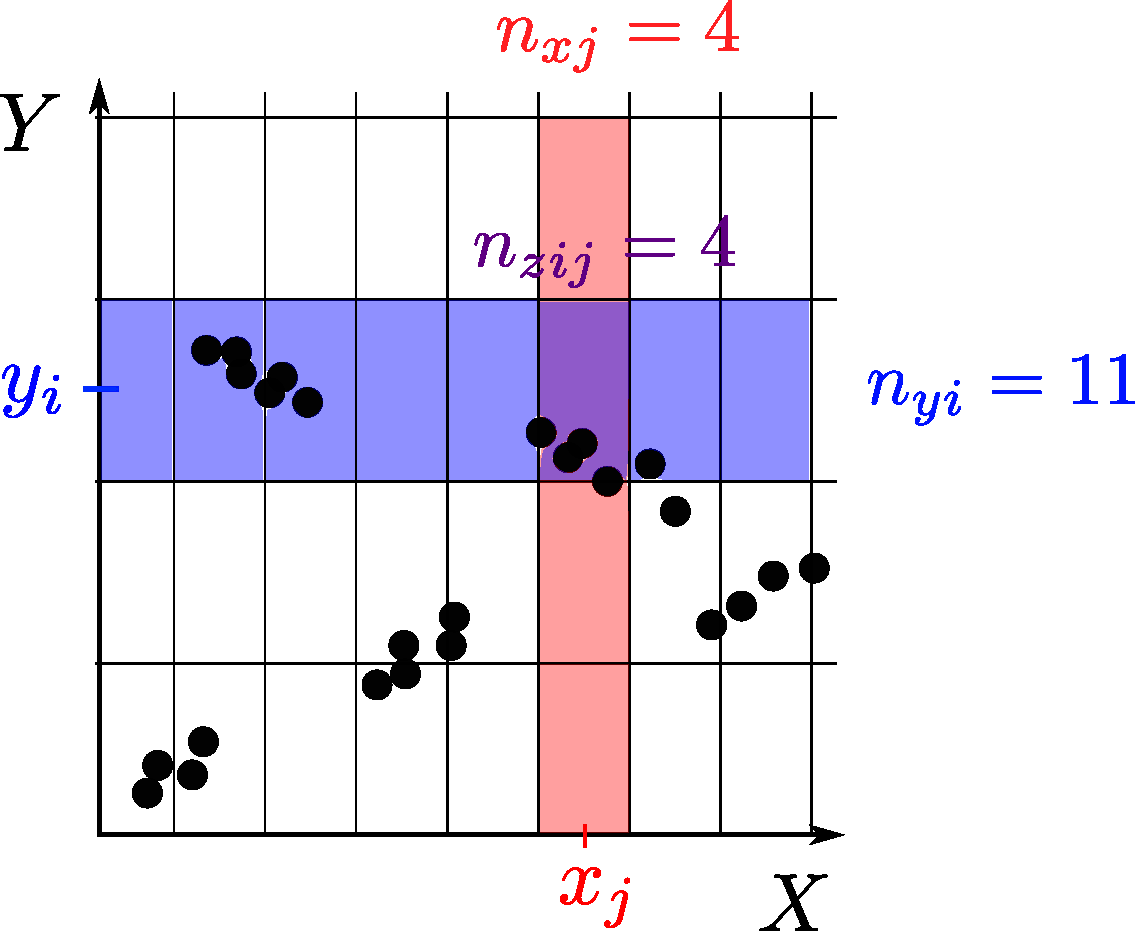
\includegraphics[width=0.3\textwidth]{boxes}
\caption{Procédé de binning pour estimer les distributions des variables $\bmu$ et $U$}
\label{fig:binning} 
\end{figure}

\section{Correlation ration}


\section{Expériences et résultats}

chap suivant ? 
